\section{Estimación del fondo de jets falseando fotones}
\label{sec:bkg:estimation}

Los principales fondos encontrados para este análisis son aquellos en los que hay al menos un fotón y un jet en el estado final. Aunque los eventos \ac{SM} \gammajet (fotones prompt discutidos en \Sect{\ref{subsec:theory:sm:prompt_photon}}) son el fondo dominante, los eventos de jets falseando fotones son otra fuente importante de fondo que hay que tener en cuenta.




Los jets pueden ser identificados erróneamente como fotones (fotones falsos) si contienen un \pizero muy energético, dando lugar a un objeto \ac{EM} indistinguible de un fotón real y altamente energético (también llamado fotón prompt). Para hacer frente a los grandes fondos conteniendo jets se aplica el criterio de identificación \texttt{Tight} a los candidatos a fotón. Se espera que esta selección contenga fotones prompt con una contaminación de jet moderada. Como no se espera que esta tasa de identificación errónea se modele con precisión en \ac{MC}, se ha utilizado un método basado en datos. La identificación offline \texttt{Tight} es por diseño más ajustada que el trigger de fotones usado para recolectar los datos, por lo que hay una fracción no despreciable de jets candidatos a fotones que fallan el \ac{WP} \texttt{Tight} pero satisfacen alguna selección intermedia. Estos jets similares a fotones, a partir de ahora llamados pseudofotones (o \texttt{Non-Tight}), se definen como aquellos que pasan la identificación \texttt{Loose} pero fallan (al menos) uno de los cortes en las siguientes \acp{SS} utilizadas en la identificación \texttt{Tight}~\cite{ATLAS-EGamma-Performance-2015-2017}: \wone, \fside, \deltae y \eratio.

Para estimar el número de jets falseando fotones en las regiones de señal del presente análisis se emplea una combinación de dos métodos. Utilizando el método ABCD con las diferentes distribuciones de aislamiento calorimétrico de fotones reales y falsos es posible estimar lo que se conocen como \acp{FaF} que permiten obtener el número de fotones falsos en las regiones de señal~\cite{ATLAS-SUSY-PhotonMetX-13TeV,ATLAS-SUSY-PhotonMetX-13TeV-NOTE,ATLAS-SUSY-PhotonJetMet-13TeV,ATLAS-SUSY-PhotonJetMet-13TeV-NOTE}. El segundo método permite contar correctamente el número de fotones reales y falsos en las regiones delimitadas por el método ABCD, haciendo uso de un procedimiento secuencial de ajustes a la distribución de aislamiento de fotones en datos y \ac{MC}.

\begin{table}[ht!]
    \centering
    \caption{Selección de eventos utilizada para los estudios de jets falseando fotones utilizando el método ABCD y ajustes a las variables de \etiso. En la \Eqn{\ref{eq:objects:egamma:iso:definitions}} se define la expresión  de \ptiso.}
    \begin{tabular}{ l  c }
        \toprule
                                & Selección \\
        \midrule
        Trigger                 & HLT\_g140\_loose \\
        \ngamma                 & \(\ge1\) \\
        \ptgam [GeV]            & \(>150\) \\
        \ptjet [GeV]            & \(> 60\) \\
        \njets                  & \(>0\) \\
        \nlep                   & \(0\) \\
        Aislamiento de trazas   & \(\ptiso < 0.05\) \\
        \(|\etagam|\)           & \(\abseta < 1.37\) o \(1.52 < \abseta < 2.37\) \\
        \myj [GeV]              & \(\myj > 500\) \\
        \bottomrule
    \end{tabular}
    \label{tab:bkg:estimation:selection}
\end{table}

Para este estudio se utilizan fotones identificados con el \ac{WP} \texttt{Loose} y no aislados. Una descripción completa de la selección de eventos utilizada se encuentra en la \Tab{\ref{tab:bkg:estimation:selection}}.
Es importante señalar que los fotones \texttt{Tight} y aislados utilizados en la búsqueda son sólo un subconjunto de los utilizados en este estudio de estimación del fondo. Al requerir que los fotones \texttt{Loose} no aislados pasen la selección mostrada en la \Tab{\ref{tab:bkg:estimation:selection}} y además pasen la identificación \texttt{Tight} y \(\etiso < 0 ~\gev\) (ver la \Eqn{\ref{eq:objects:egamma:iso:definitions}}), se recuperan los fotones \texttt{Tight} y aislados utilizados en la búsqueda.
Finalmente se lleva a cabo un procedimiento manual de eliminaciones de objetos superpuestos entre los fotones y los jets para eliminar el jet solapado con el fotón \texttt{Loose} si \(\dryj<0.4\).

Este método se lleva a cabo utilizando datos, pero, dado que el \textit{unblinding} de los datos completos del Run-2 no se realiza hasta la última etapa del análisis, sólo se utiliza el conjunto de datos de 2015+2016, ya que ya fue observado en un trabajo anterior de la colaboración \ac{ATLAS}~\cite{ATLAS-PhotonJetResonances-2016}.


\subsection{Método ABCD}
\label{subsec:bkg:estimation:abcd}

El método ABCD define una región de señal \(A\) y tres regiones de control: \(B\), \(C\) y \(D\).
Estas regiones se definen variando el estado de identificación entre \texttt{Tight} y \texttt{Non-Tight}, y también cambiando los requisitos de aislamiento calorimétrico (aislado y no aislado)~\cite{ATLAS-EXOTICS-Monophoton-2017}.
La definición completa de las regiones ABCD es la siguiente
\begin{itemize}
    \item Región \(A\): Fotones \texttt{Tight} y \(\etiso < 0~ \gev\),
    \item Región \(B\): Fotones \texttt{Tight} y \(\etiso > 8~ \gev\),
    \item Región \(C\): Fotones \texttt{Non-Tight} y \(\etiso < 0~ \gev\),
    \item Región \(D\): Fotones \texttt{Non-Tight} y \(\etiso > 8~ \gev\),
\end{itemize}
donde \etiso se definió en la \Eqn{\ref{eq:objects:egamma:iso:definitions}}. La \Fig{\ref{fig:bkg:estimation:abcd:diagram}} muestra las cuatro regiones diferentes resultantes.

\begin{figure}[ht!]
    \centering
    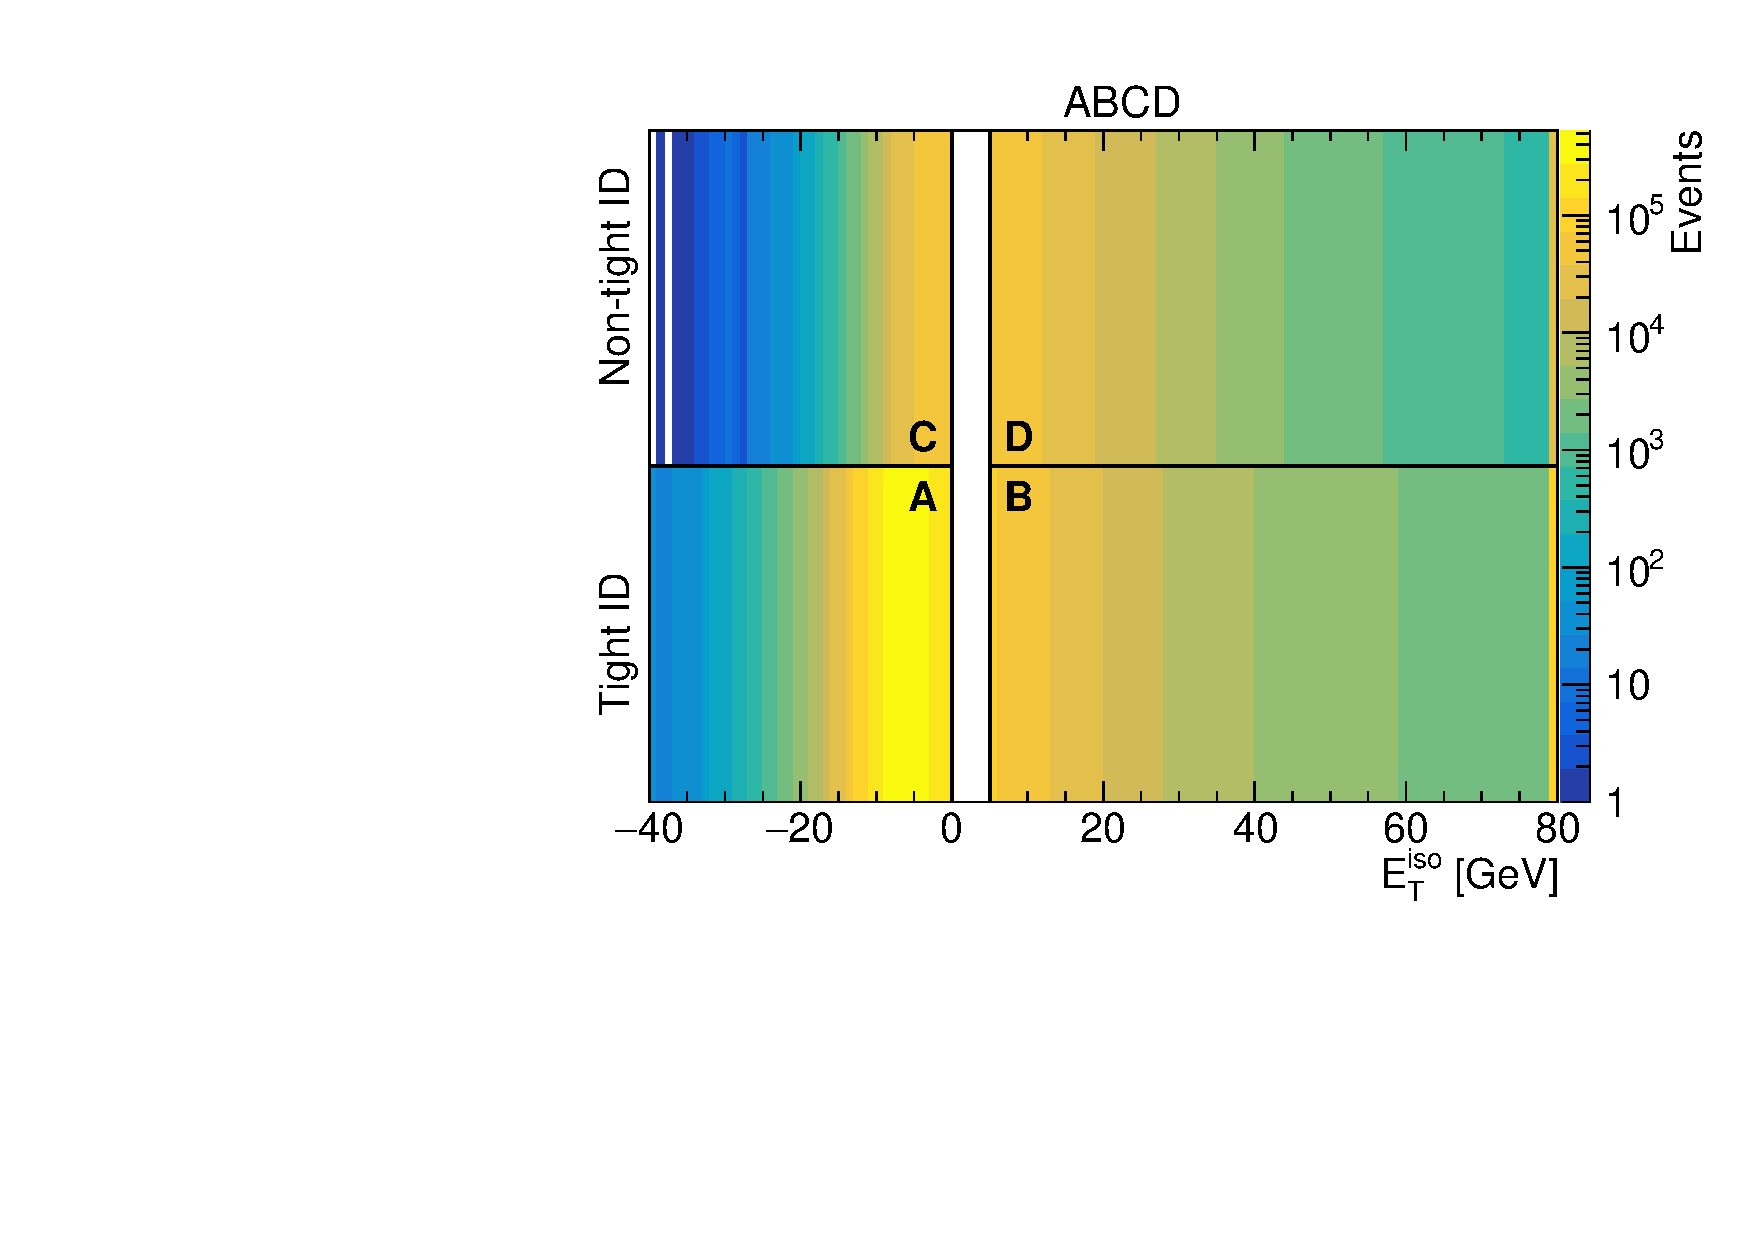
\includegraphics[width=0.65\textwidth]{5_resonances/bkg/estimation/ABCD_data_regions}
    \caption{Distribución bidimensional en el plano de identificación vs. \etiso obtenida de los datos.}
    \label{fig:bkg:estimation:abcd:diagram}
\end{figure}

Suponiendo que no hay contaminación de señal en ninguna región de control, las regiones \(B\), \(C\) y \(D\) sólo se componen de fondo \(N_{(B,C,D)}=N^{b}_{(B,C,D)}\). Además, suponiendo que no existe correlación entre el aislamiento y las \acp{SS} consideradas, se cumple la siguiente relación \(N^{b}_{B}/N^{b}_{A}=N^{b}_{D}/N^{b}_{C}\). Des esta forma, podrían definirse dos \acp{FaF} diferentes:
\begin{equation*}
    \ffiso = \frac{N_{C}}{N_{D}} \qquad \ffid = \frac{N_{B}}{N_{D}}
\end{equation*}
Por lo tanto, el número de jets que falsan fotones se puede estimar utilizando los \ac{FaF} como:
\begin{equation}
    \label{eq:bkg:estimation:abcd:njfakes}
    N_{\jfake} = N_{A} = \ffiso \times N_{B}  = \ffid \times N_{C}.
\end{equation}

Se podrían utilizar dos enfoques diferentes: modelar los fotones falsos utilizando fotones \texttt{Tight} pero no aislados de la región \(B\) utilizando los \ffiso, o modelar los fotones falsos utilizando el fotones \texttt{Non-Tight} pero aislados usando los \ffid.
Aunque ambos enfoques dan resultados equivalentes, se utiliza el enfoque \ffiso ya que conduce a estadísticas más altas.


Utilizando el \ac{FaF}, ahora es posible estimar la contribución de fondo de los jets falseando fotones en cada región del análisis (\(X\)). Para ello, se define una región de control de jets (CRJ-X) igual a la región \(X\) pero sustituyendo los requisitos de aislamiento por los utilizados en la región \(B\), y pesada por el correspondiente \ffiso:
\begin{equation*}
    N^{X}_{\jfake}(\pt) = \ffiso(\pt)\cdot N_{\text{CRJ-X}}(\pt)
\end{equation*}





\subsection{Correcciones al método de ABCD}
\label{subsec:bkg:estimation:abcd_corrections}

Deben aplicarse varias correcciones al método ABCD.
La primera consiste en considerar la posibilidad de una contaminación de señal en cualquiera de las regiones de control \(B\), \(C\) o \(D\) (fotones filtrados). Restando la cantidad de eventos de señal en estas regiones, la \Eqn{\ref{eq:bkg:estimation:abcd:njfakes}} se convierte en:
\begin{equation}
    \label{eq:bkg:estimation:abcd_corrections:njfakes_leak}
    N_{\jfake} = \frac{N_{B} - N_{B}^{s}}{N_{D} - N_{D}^{s}} \times (N_{C} - N_{C}^{s})
\end{equation}
donde \(N_{(B,C,D)}^{s}\) es el número de fotones reales en cada región. La estimación de estos números es una tarea complicada ya que se necesita para tener una descripción correcta de los fotones reales en los datos y está altamente contaminada con fotones falsos. El cálculo del número de fotones reales en los datos se realiza con un método de ajustes secuenciales a la distribución de aislamiento calorimétrico en los datos, que se explica con más detalle a continuación.


La presencia de una correlación residual del fondo en las cuatro regiones que puede manifestarse como una diferencia en las distribuciones del fondo para las regiones \texttt{Tight} y \texttt{Non-Tight} podría tenerse en cuenta calculando:
\begin{equation*}
    R = \frac{N^{b}_{A}\,N^{b}_{D}}{N^{b}_{B}\,N^{b}_{C}} \neq 1.
\end{equation*}
Sin embargo, como \(R\) no se puede encontrar en los datos porque eso significaría obtener \(N_A\) (es decir, mirar los datos en la región de se\~nal), se calcula un parámetro equivalente, que también se puede escribir utilizando teniendo en cuenta los fotones reales en las regiones de control:
\begin{equation*}
    R' = \frac{N_{A'}\,N_{D'}}{N_{B'}\,N_{C'}} = \frac{(N_{A'} - N^{s}_{A'})\,(N_{D'}-N^s_{D'})}{(N_{B'}-N^s_{B'})\,(N_{C'}-N^s_{C'})}
\end{equation*}
con la definición para cada región siendo:
\begin{itemize}
    \item región \(A'\): Fotones \texttt{Tight} y \(8 < \etiso < 15~ \gev\).
    \item región \(B'\): Fotones \texttt{Tight} y \(16 < \etiso < 80~ \gev\).
    \item región \(C'\): Fotones \texttt{Non-Tight} y \(8 < \etiso < 15~ \gev\).
    \item región \(D'\): Fotones \texttt{Non-Tight} y \(16 < \etiso < 80~ \gev\).
\end{itemize}
La selección particular de 8 \gev\ pretende definir una región sólo de fondo, pero manteniendo suficientes estadística para calcular los valores de \(R'\). En la \Fig{\ref{fig:bkg:estimation:abcd_corrections:rprime}} se muestran los valores \(R'\) en función de \ptgam.
Los valores están muy próximos a 1, con algunas excepciones en las que los valores se desvían de 1 en una cantidad máxima de \(\approx 20\%\) a bajo \ptgam.
\begin{figure}[htbp]
    \centering
    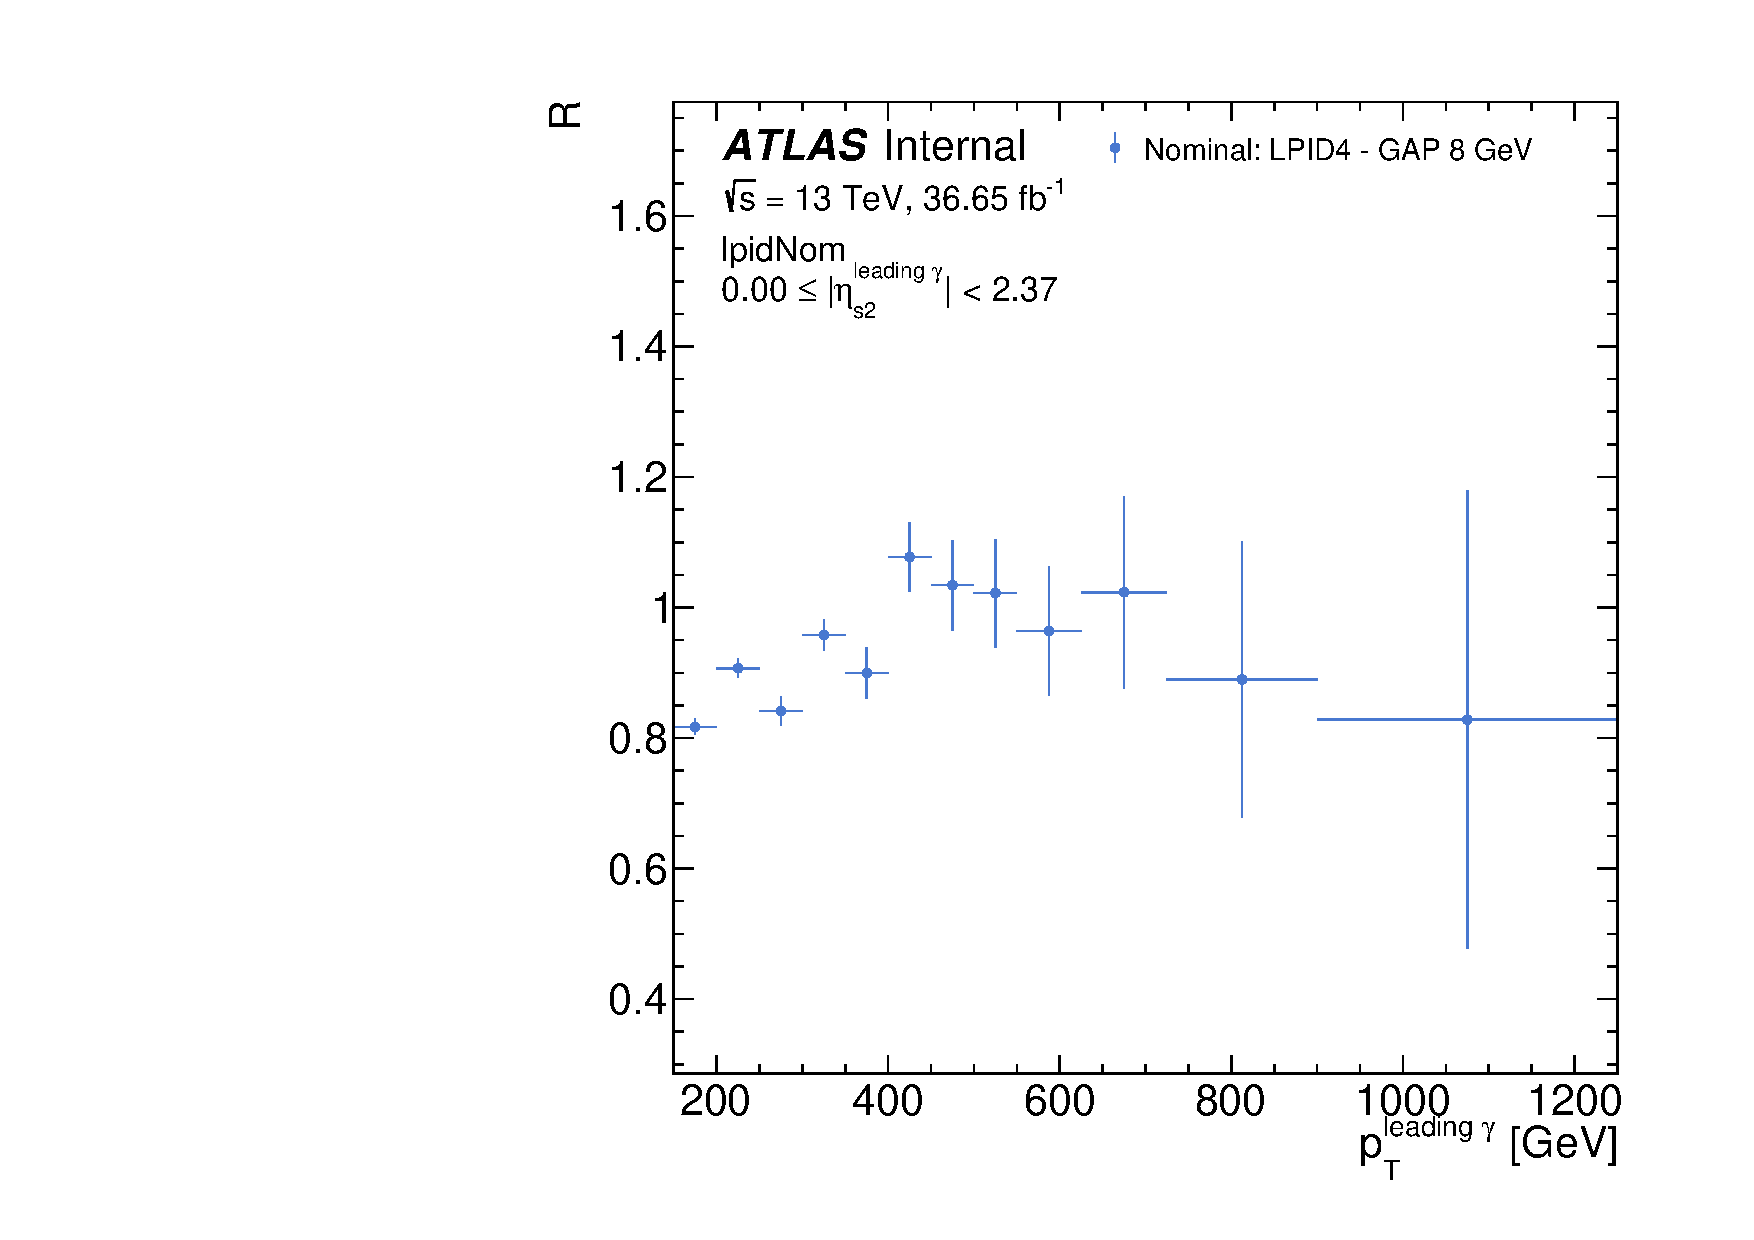
\includegraphics[width=0.5\linewidth]{5_resonances/bkg/estimation/coefficients/can__R__lpidNom__lph_pt0__abslph_etas20_0__2015_2016}
    \caption{Valores medidos de \(R'\) en función de \ptgam. Las barras de error muestran el error estadístico.}
    \label{fig:bkg:estimation:abcd_corrections:rprime}
\end{figure}

Por último, teniendo en cuenta los fotones filtrados en las regiones de control y las posibles correlaciones, la \Eqn{\ref{eq:bkg:estimation:abcd_corrections:njfakes_leak}} resulta, para el número esperado jets falseando fotones:
\begin{equation}
    \label{eq:bkg:estimation:abcd_corrections_ffiso}
    N_{\jfake}(\pt) =
    N^{b}_{A} =
    \left[R'  \frac{N_{C}-N^{s}_{C}}{N_{D}-N^{s}_{D}}  \left(1 - \frac{N^{s}_{B}}{N_{B}} \right)\right] \times N_B = \ffiso(\pt)  \times  N_{B}(\pt).
\end{equation}






\subsection{Procedimiento de ajustes al aislamiento calorimétrico}
\label{subsec:bkg:estimation:fits}


Para estimar el número de jets falseando fotones en las regiones de señal del análisis es necesario tener una estimación del número de eventos con fotones reales en las regiones de control del ABCD: regiones \(B\), \(C\) y \(D\). Para ello, se realiza una serie de ajustes a la distribución de aislamiento de los datos y de fotones reales obtenidos por \ac{MC}, tanto para fotones \texttt{Tight} como \texttt{Non-Tight}. El objetivo final de los ajustes secuenciales es contar con las componentes de fotones reales y falsos de los datos, que luego se utilizarán para calcular el número de fotones reales en las regiones de control del ABCD. El procedimiento utiliza las muestras de \ac{MC} de las que se espera que únicamente contengan fotones reales. El cálculo se realiza en 11 bines de \ptgam:
\begin{equation*}
    \ptgam: \left[ 150, 200, 250, 300, 350, 400, 450, 500, 550, 625, 725, 900, \infty \right]~\gev.
\end{equation*}


La forma del aislamiento calorimétrico \etiso se ajusta de forma secuencial utilizando fotones que pasan los criterios de identificación \texttt{Tight} y \texttt{Non-Tight}, como se ha explicado anteriormente.
Por definición, los eventos con \(\etiso<0~\gev\) pasan el criterio de aislamiento calorimétrico y corresponden a fotones que caen en la región \(A\) si son \texttt{Tight} o \(C\) si son \texttt{Non-Tight}. Por otro lado, los eventos con \(\etiso>0~\gev\) definen las regiones \(B\) (fotones \texttt{Tight}) y \(D\) (fotones \texttt{Non-Tight}).
Tanto los fotones \texttt{Tight} como los \texttt{Non-Tight} contendrán un componente de fotones falsos que dominará sobre los fotones filtrados en el último caso~\cite{ATLAS-DiPhotonSearchIsolation-NOTE,ATLAS-EleMuPhoIsolation-NOTE}.

La secuencia de ajustes es la siguiente:
\begin{enumerate}
    \item \underline{Ajuste de fotones \texttt{Tight} en \ac{MC}}: Dado que las muestras de fotones prompt proporcionan una buena descripción de los fotones \texttt{Tight}, su distribución de \etiso se ajusta con una función \ac{CBall}\footnote{Esta función consiste en una función Gaussian pero una de las colas de ella está descripta por una forma funcional que sigue la ley de potencia.}. Se encontró que la simple descripción \ac{CBall} no se acomoda bien en toda el rango ajustado, especialmente en la zona del pico de la distribución de \etiso, por lo tanto se requiere de una función más flexible. De este modo, se utiliza una versión mejorada de la \ac{CBall}: la \ac{DSACB}\footnote{Como su nombre sugiere, en una \ac{DSACB}, las dos colas se modelan mediante funciones que siguen de ley de potencia, y el núcleo de la distribución gaussiana tiene dos desviaciones estándar diferentes, de ahí la asimetría.}.
    % Aunque la descripción es mucho mejor en este caso, el núcleo gaussiano sigue teniendo dificultades para modelar correctamente el pico de la distribución.
    \item \underline{Fotones filtrados}: La forma de los fotones falsos se estima sustrayendo la componente de fotones filtrados (obtenida de la simulación \ac{MC}) a los datos en todo el rango \etiso. Esto proporciona una descripción muy buena de la componente de fotones falsos en las regiones \texttt{Non-Tight} (eso es, regiones \(C\) y \(D\)).
    \item \underline{Ajuste combinado a los datos en regiones \texttt{Tight}}: Utilizando la forma de fotones reales brindada por la función \ac{DSACB} estimada en el primer paso y la forma de fotones falsos estimada en el paso anterior, se realiza un ajuste combinado a la distribución \etiso de fotones \texttt{Tight} de los datos. Ejemplos del ajuste resultante en tres bines de \pt se muestran en la \Fig{\ref{fig:bkg:estimation:fits_tightID_data}}.
    
        La distribución final concuerda bien con los datos, lo que indica la correcta selección de las distribuciones para cada componente. El componente de fotones reales es el responsable del pico en valores bajos de aislamiento, mientras que las componentes de fotones falsos contribuyen principalmente en el rango \(0~\gev < \etiso < 40 ~\gev\) contribuyendo al número total de eventos mucho menos que los reales como era de esperar. Pueden observarse algunas diferencias entre el ajuste combinado y los datos cerca del pico de la distribución, que es evidente en los residuos normalizados del ajuste. Esta diferencia también se observó en el primer paso del cálculo al modelar las componentes de los fotones reales y tiene su origen directo en el modelado gaussiano del pico.

        \begin{figure}[bth!]
            \centering
            \begin{subfigure}[h]{0.32\linewidth}
                \centering
                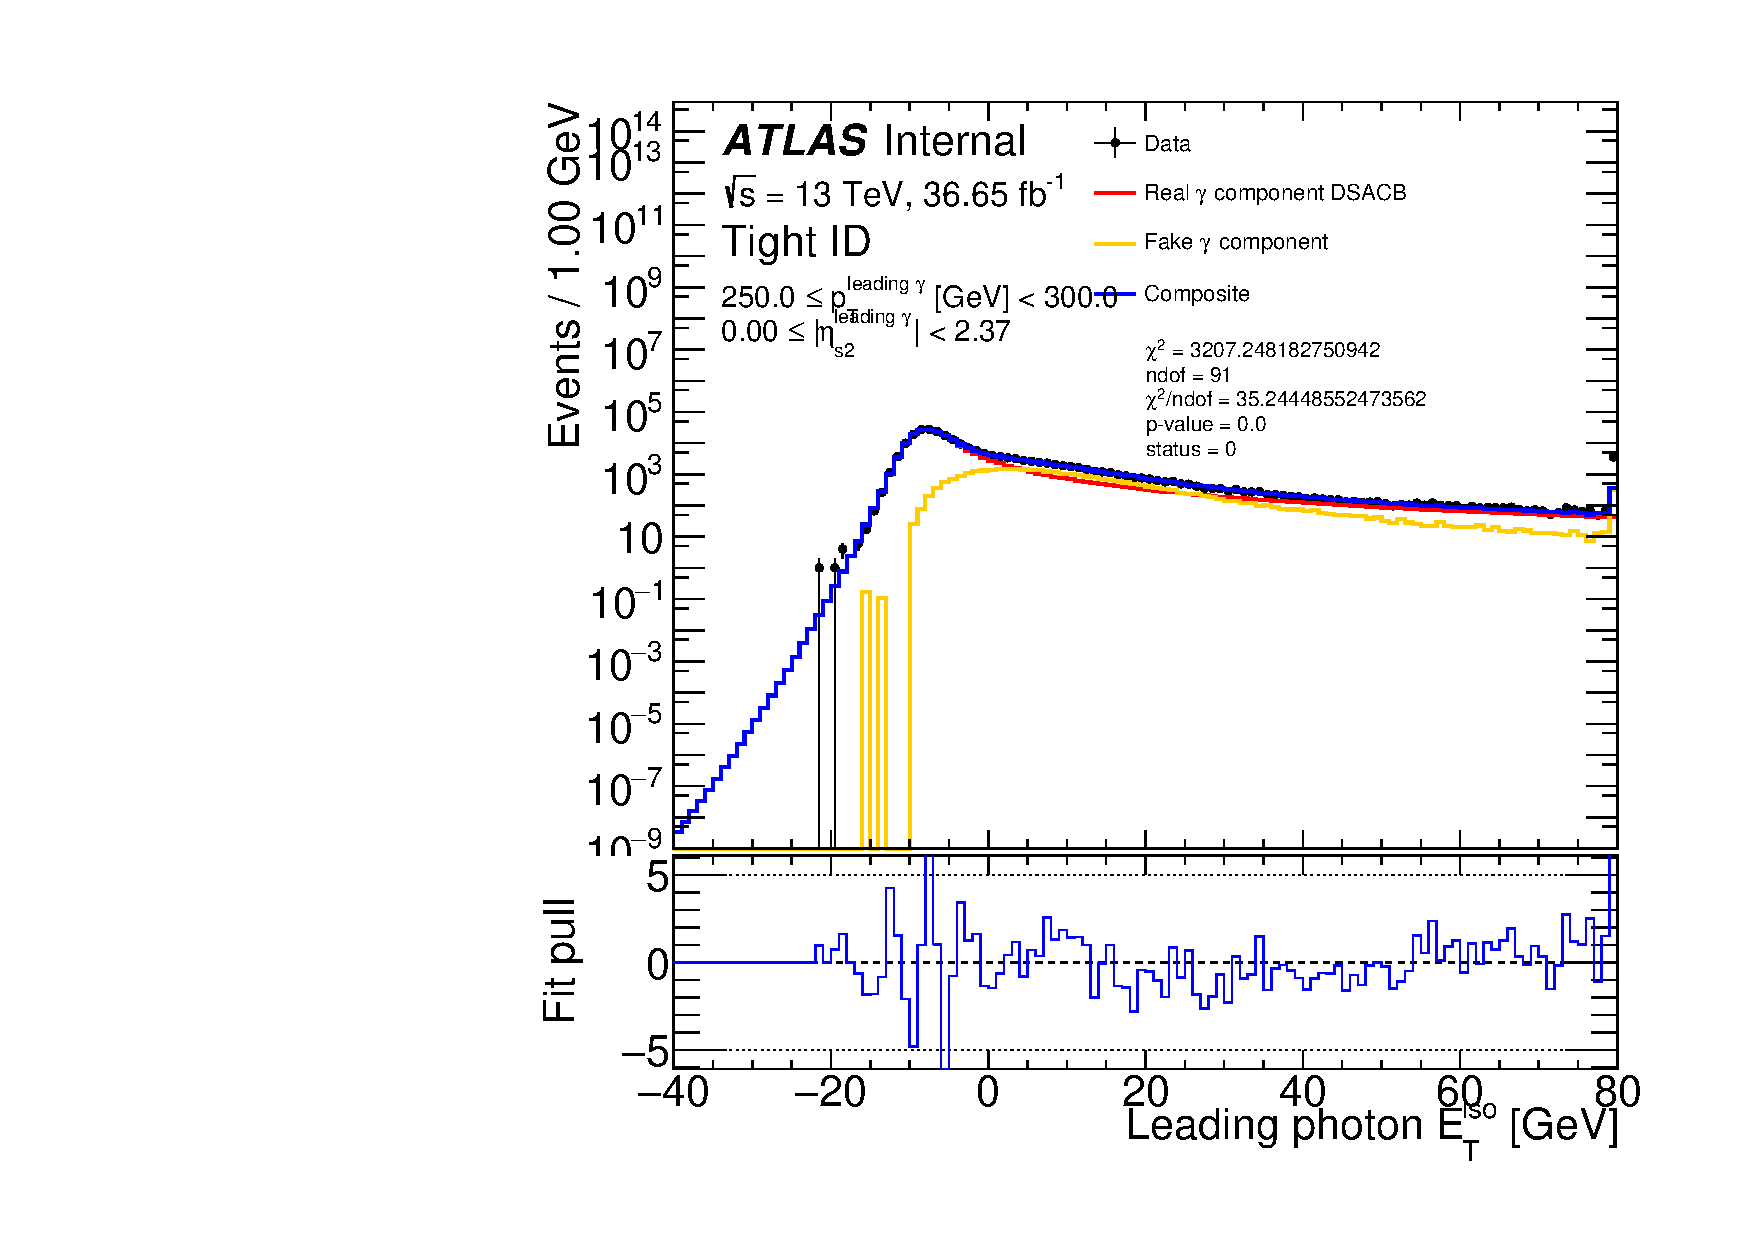
\includegraphics[width=\linewidth]{5_resonances/bkg/estimation/fits/lpid4/2015_2016/lph_pt0/lph_pt0__250p0/data__tight__composite__lph_pt0__250p0__abslph_etas20__0p00}
                \caption{\(250 < \ptgam < 300~\gev\).}
            \end{subfigure}
            \begin{subfigure}[h]{0.32\linewidth}
                \centering
                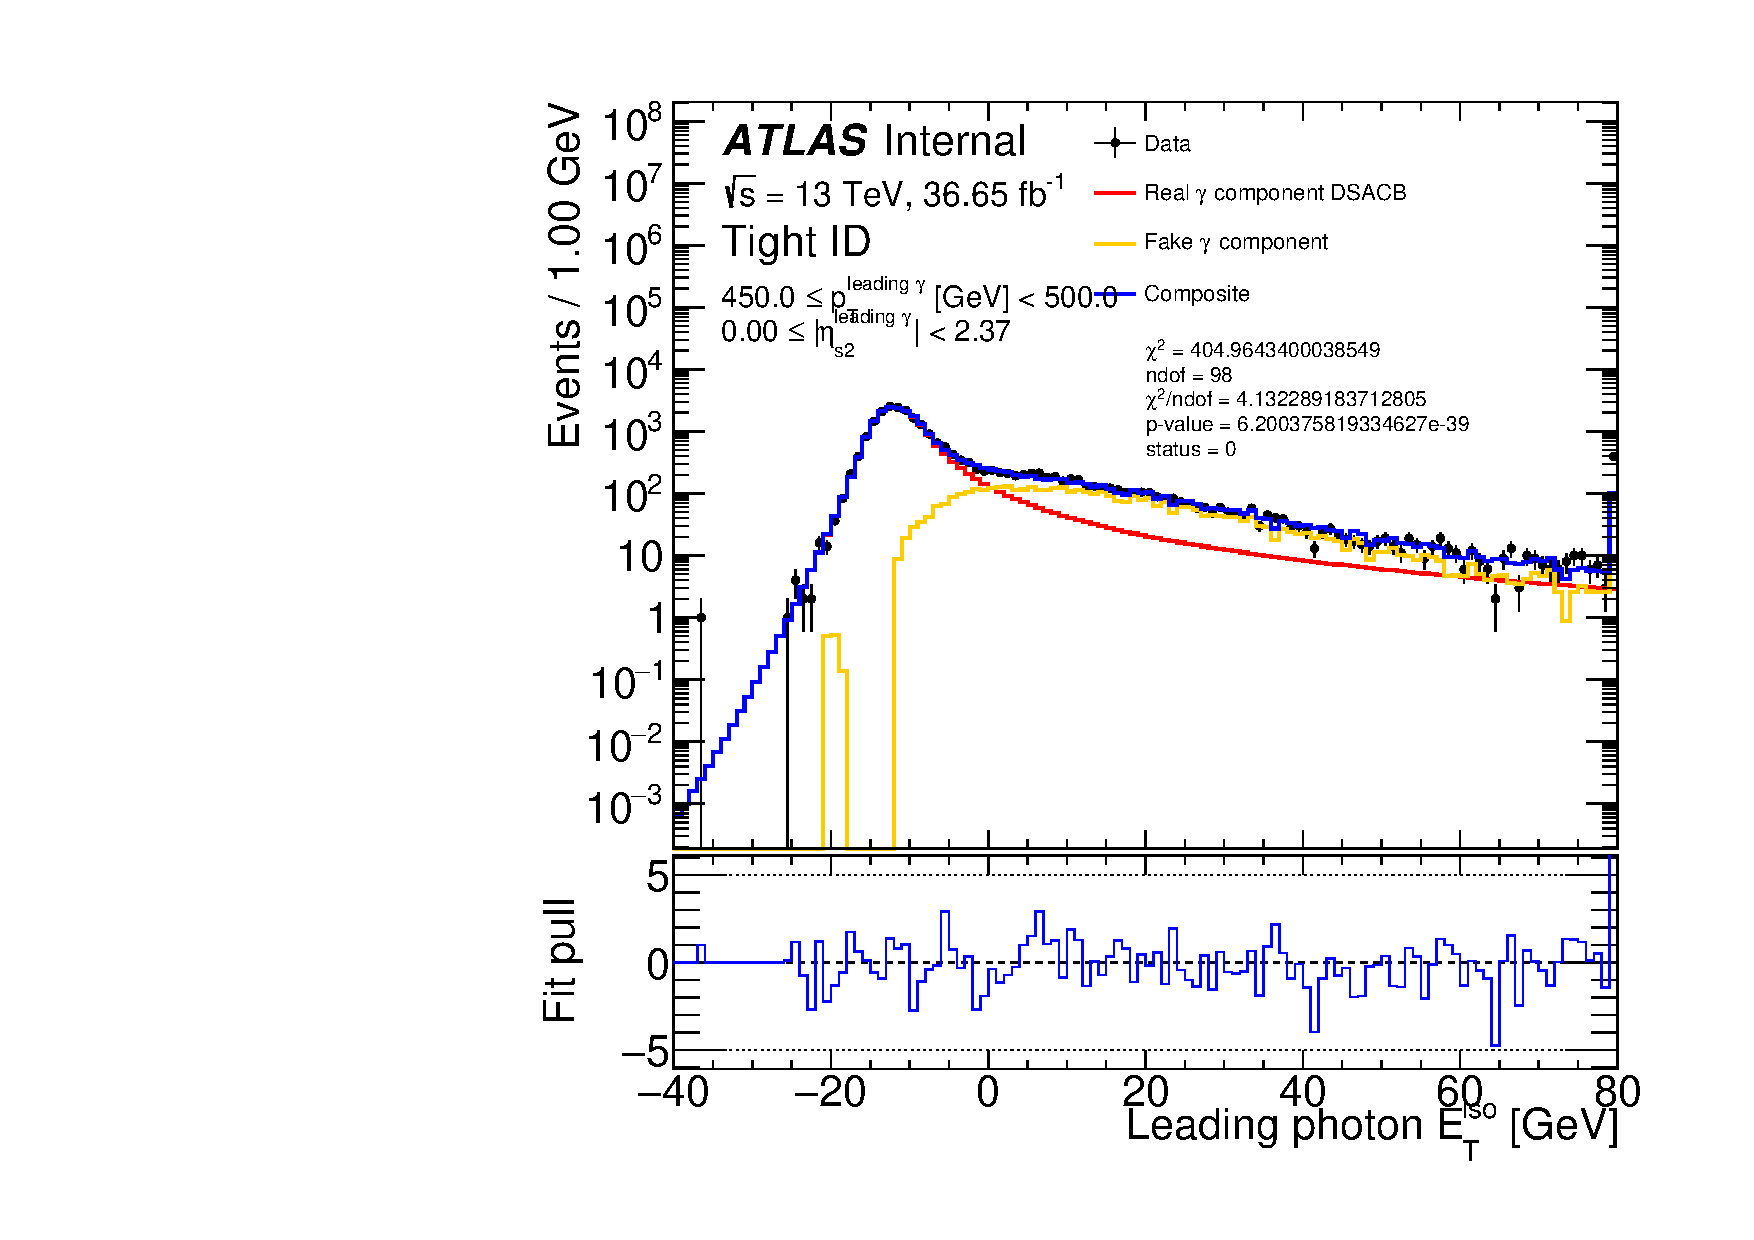
\includegraphics[width=\linewidth]{5_resonances/bkg/estimation/fits/lpid4/2015_2016/lph_pt0/lph_pt0__450p0/data__tight__composite__lph_pt0__450p0__abslph_etas20__0p00}
                \caption{\(450 < \ptgam < 500~\gev\).}
            \end{subfigure}
            \begin{subfigure}[h]{0.32\linewidth}
                \centering
                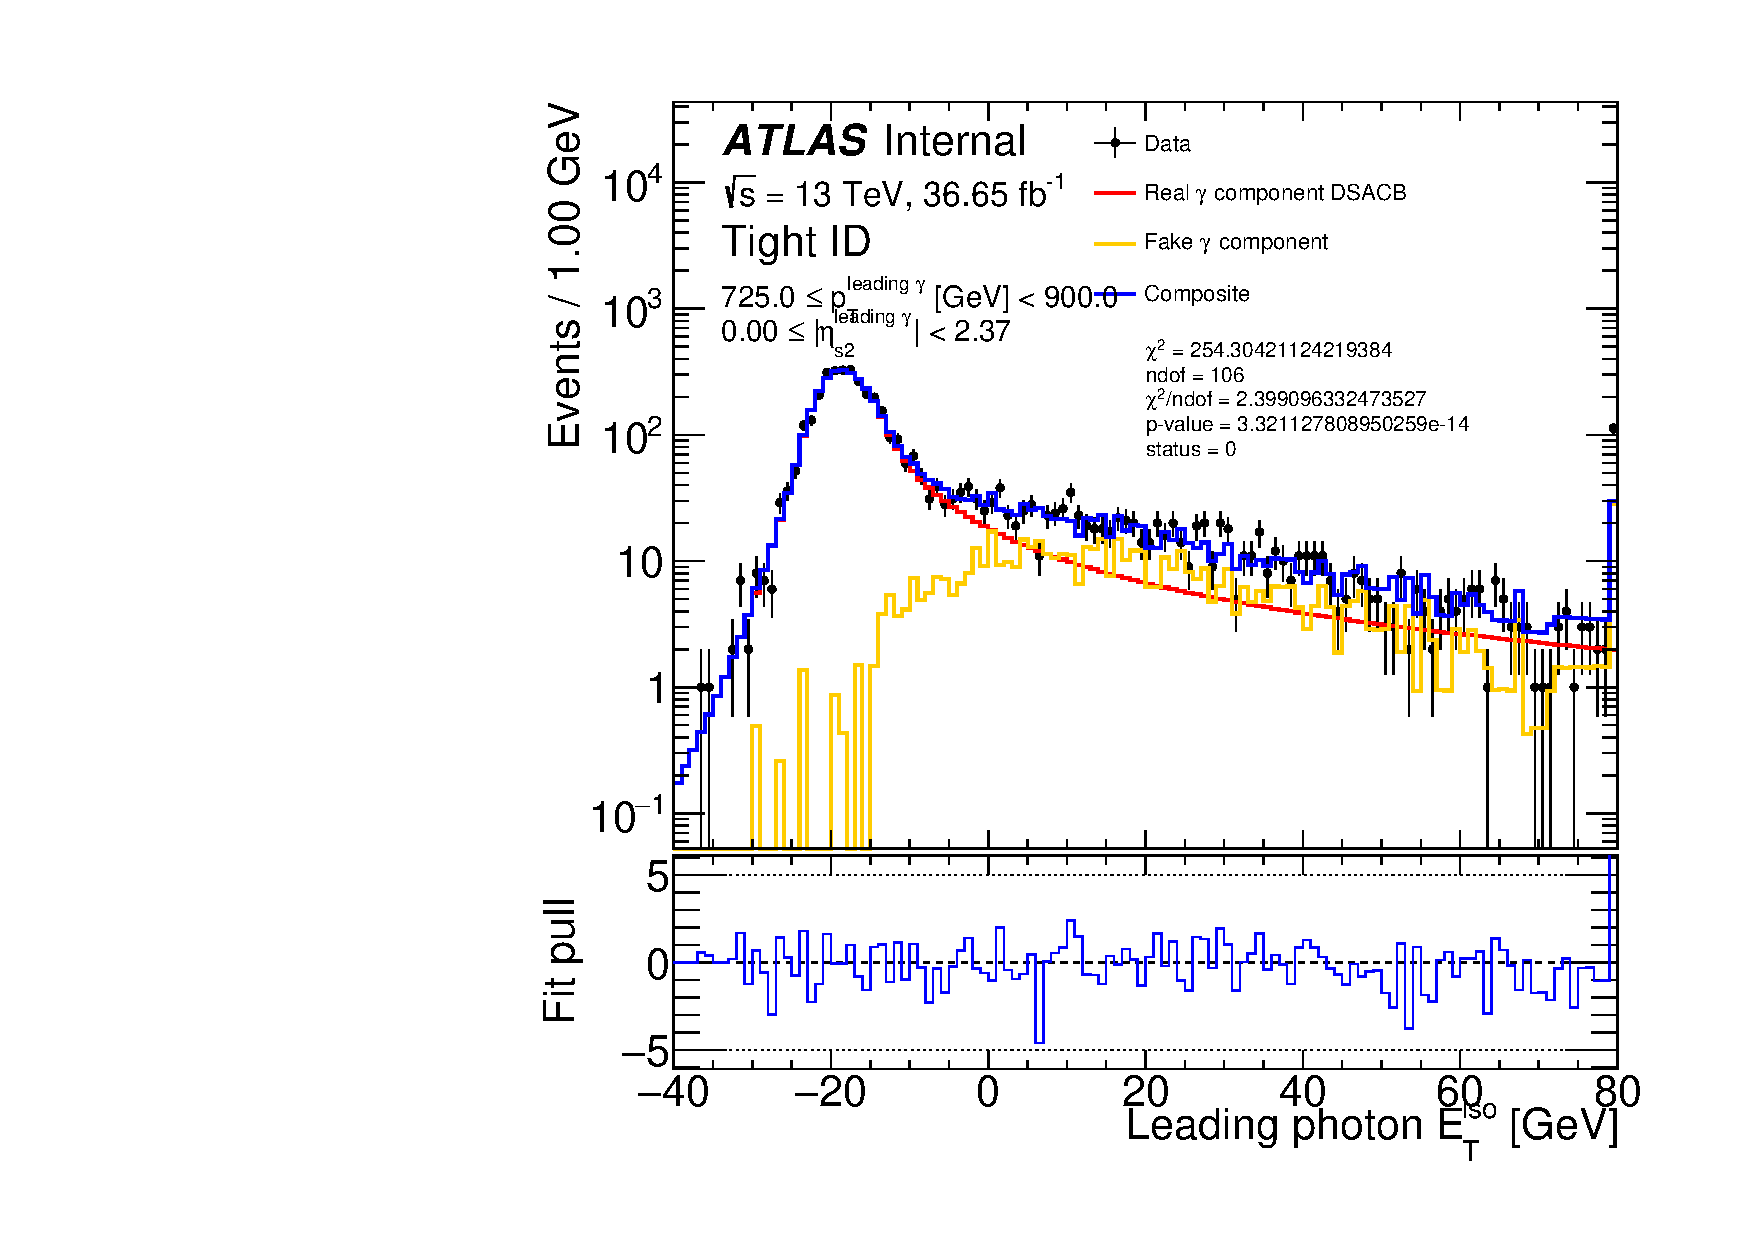
\includegraphics[width=\linewidth]{5_resonances/bkg/estimation/fits/lpid4/2015_2016/lph_pt0/lph_pt0__725p0/data__tight__composite__lph_pt0__725p0__abslph_etas20__0p00}
                \caption{\(725 < \ptgam < 900~\gev\).}
            \end{subfigure}
            \caption{Ajuste combinado a los datos. La curva roja representa la componente de fotones reales, que se representa mediante una función del tipo \ac{DSACB}, calculada en el primer paso de la secuencia de ajustes. El histograma amarillo es la contribución de los fotones falsos, obtenida en el segundo paso. El panel inferior de las figuras muestran los residuos normalizados (o pull) de los ajustes.}
            \label{fig:bkg:estimation:fits_tightID_data}
        \end{figure}
\end{enumerate}





\subsection{Resultados}
\label{subsec:bkg:estimation:results}

Del procedimiento anterior, que utiliza el método ABCD y una secuencia de ajustes usando la distribución de \etiso se pueden extraer varias cifras clave. En primer lugar, una variable importante para comprender mejor la física subyacente es la pureza de procesos \gammajet, calculada como
\[
    P_A = \frac{
        N^{A}_{\text{real}\gamma, \text{postfit}}
    }{
        N^{A}_{\text{real}\gamma, \text{postfit}} + N^{A}_{\text{fake}\gamma, \text{postfit}}
    }.
\]
Estas purezas se muestran en la \Fig{\ref{fig:bkg:estimation:results:results:purities}} y sus valores numéricos en la \Tab{\ref{tab:bkg:estimation:results:ffiso_purity_values}}. Como puede observarse, se alcanzan purezas mayores al \(92\%\) en todo el rango de \ptgam, lo que indica que los procesos que contienen un fotón real y un jet abarcan la mayor parte de la muestra, mientras que la fracción de los procesos de jet falseando fotones son menores al \(10\%\).
% Las medidas de pureza se suavizan utilizando un spline de orden \(3^{\text{rd}}\), mostrado con la línea roja en la figura.

\begin{table}[ht!]
    \caption{\acp{FaF} y purezas en función de \ptgam calculadas con los métodos descriptos previamente.}
    \begin{tabular}{lcc}
        \toprule
        \(p_{T}^{\text{leading} \gamma}\) [GeV] & \(FF_{\text{iso}}\) &  Pureza de \(\gamma\) reales en region \(A\) \\
        \midrule
        $150-200$    & $0.1873$ & $0.9201$ \\
        $200-250$    & $0.1885$ & $0.9321$ \\
        $250-300$    & $0.1901$ & $0.9418$ \\
        $300-350$    & $0.1918$ & $0.9494$ \\
        $350-400$    & $0.1934$ & $0.9552$ \\
        $400-450$    & $0.1948$ & $0.9593$ \\
        $450-500$    & $0.1956$ & $0.9620$ \\
        $500-550$    & $0.1956$ & $0.9636$ \\
        $550-625$    & $0.1943$ & $0.9642$ \\
        $625-725$    & $0.1891$ & $0.9633$ \\
        $725-900$    & $0.1703$ & $0.9604$ \\
        $900-\infty$ & $0.0835$ & $0.9650$ \\
        \bottomrule
    \end{tabular}
    \label{tab:bkg:estimation:results:ffiso_purity_values}
    \centering
\end{table}




\begin{figure}[ht!]
    \centering
    \begin{subfigure}[h]{0.49\linewidth}
        \centering
        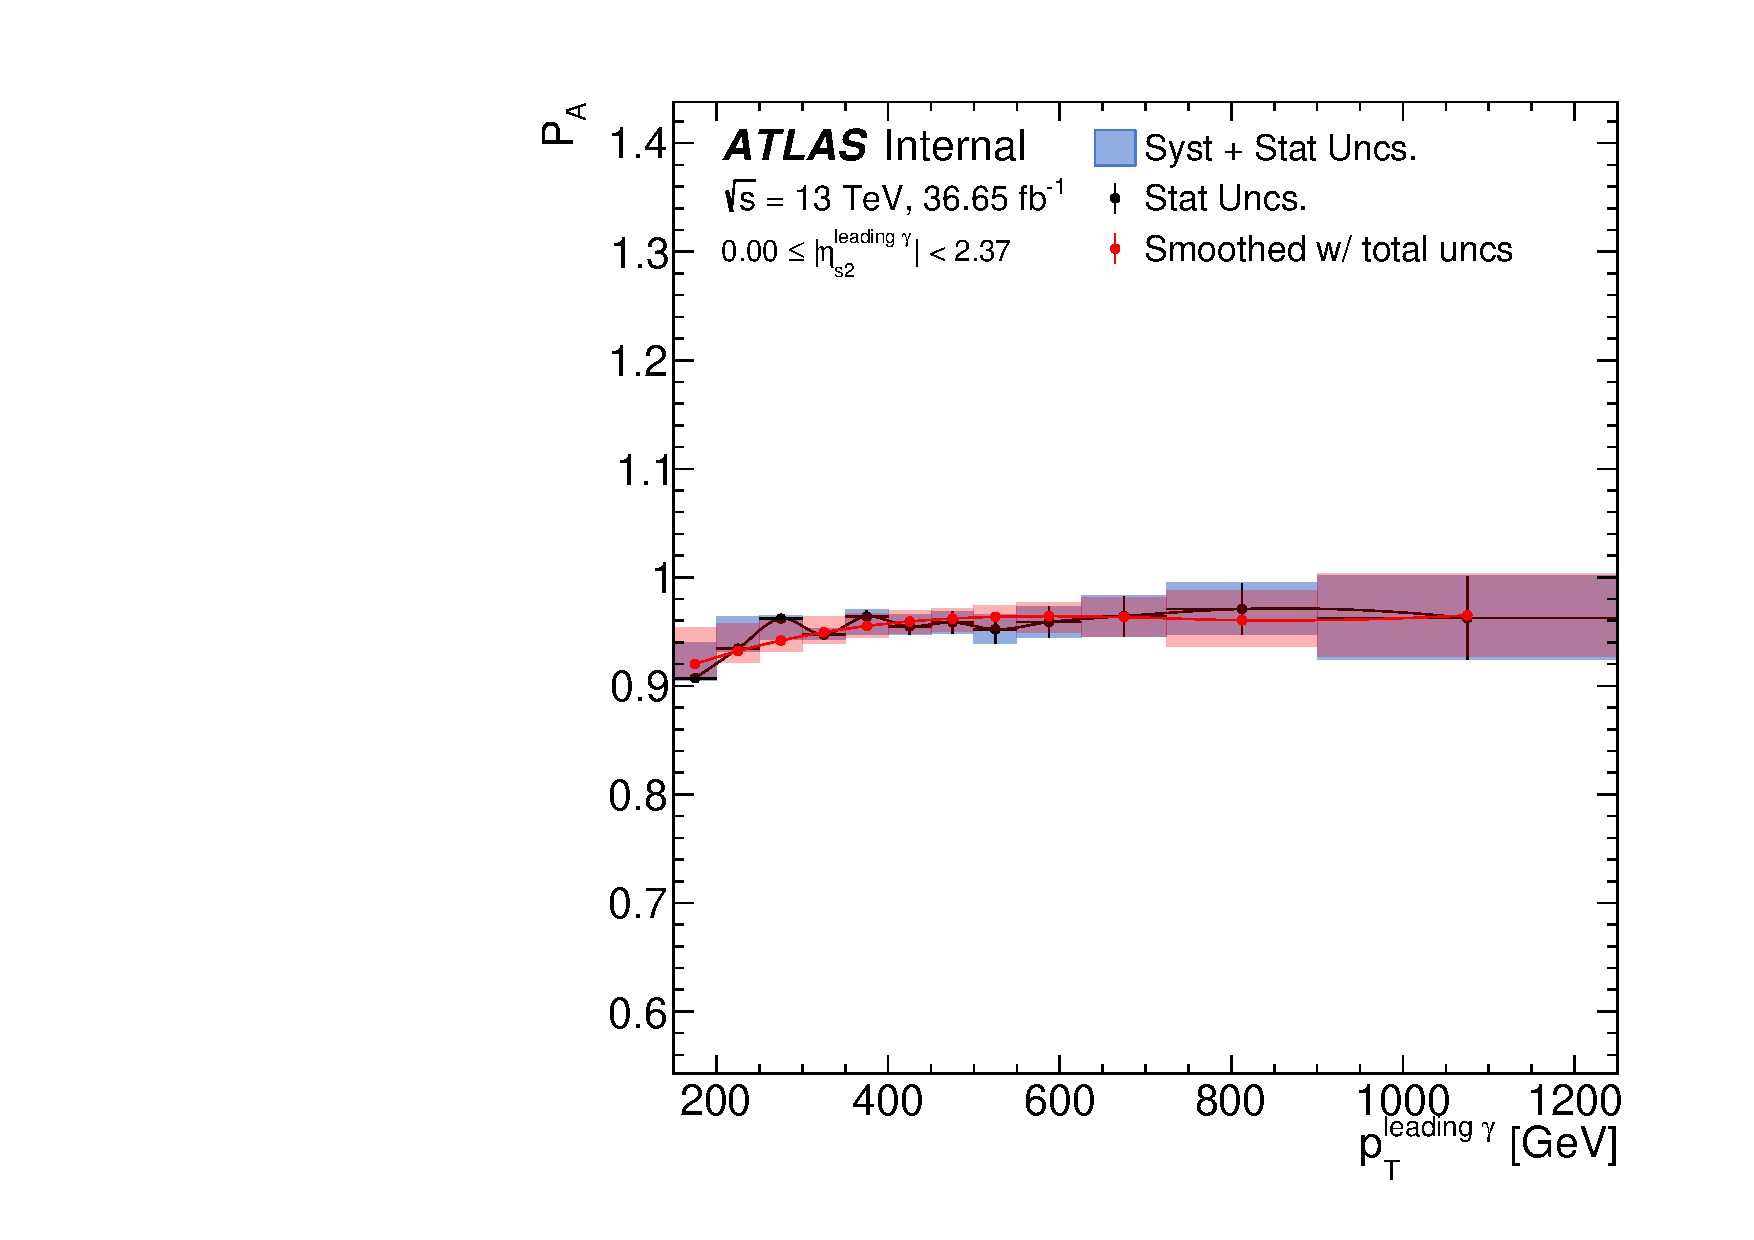
\includegraphics[width=\linewidth]{5_resonances/bkg/estimation/coefficients/can__purity_real_A__withsysts__lph_pt0__abslph_etas20_abslph_etas20__0p00__2015_2016}
        \caption{\(P_A\).}
        \label{fig:bkg:estimation:results:results:purities}
    \end{subfigure}
    \hfill
    \begin{subfigure}[h]{0.49\linewidth}
        \centering
        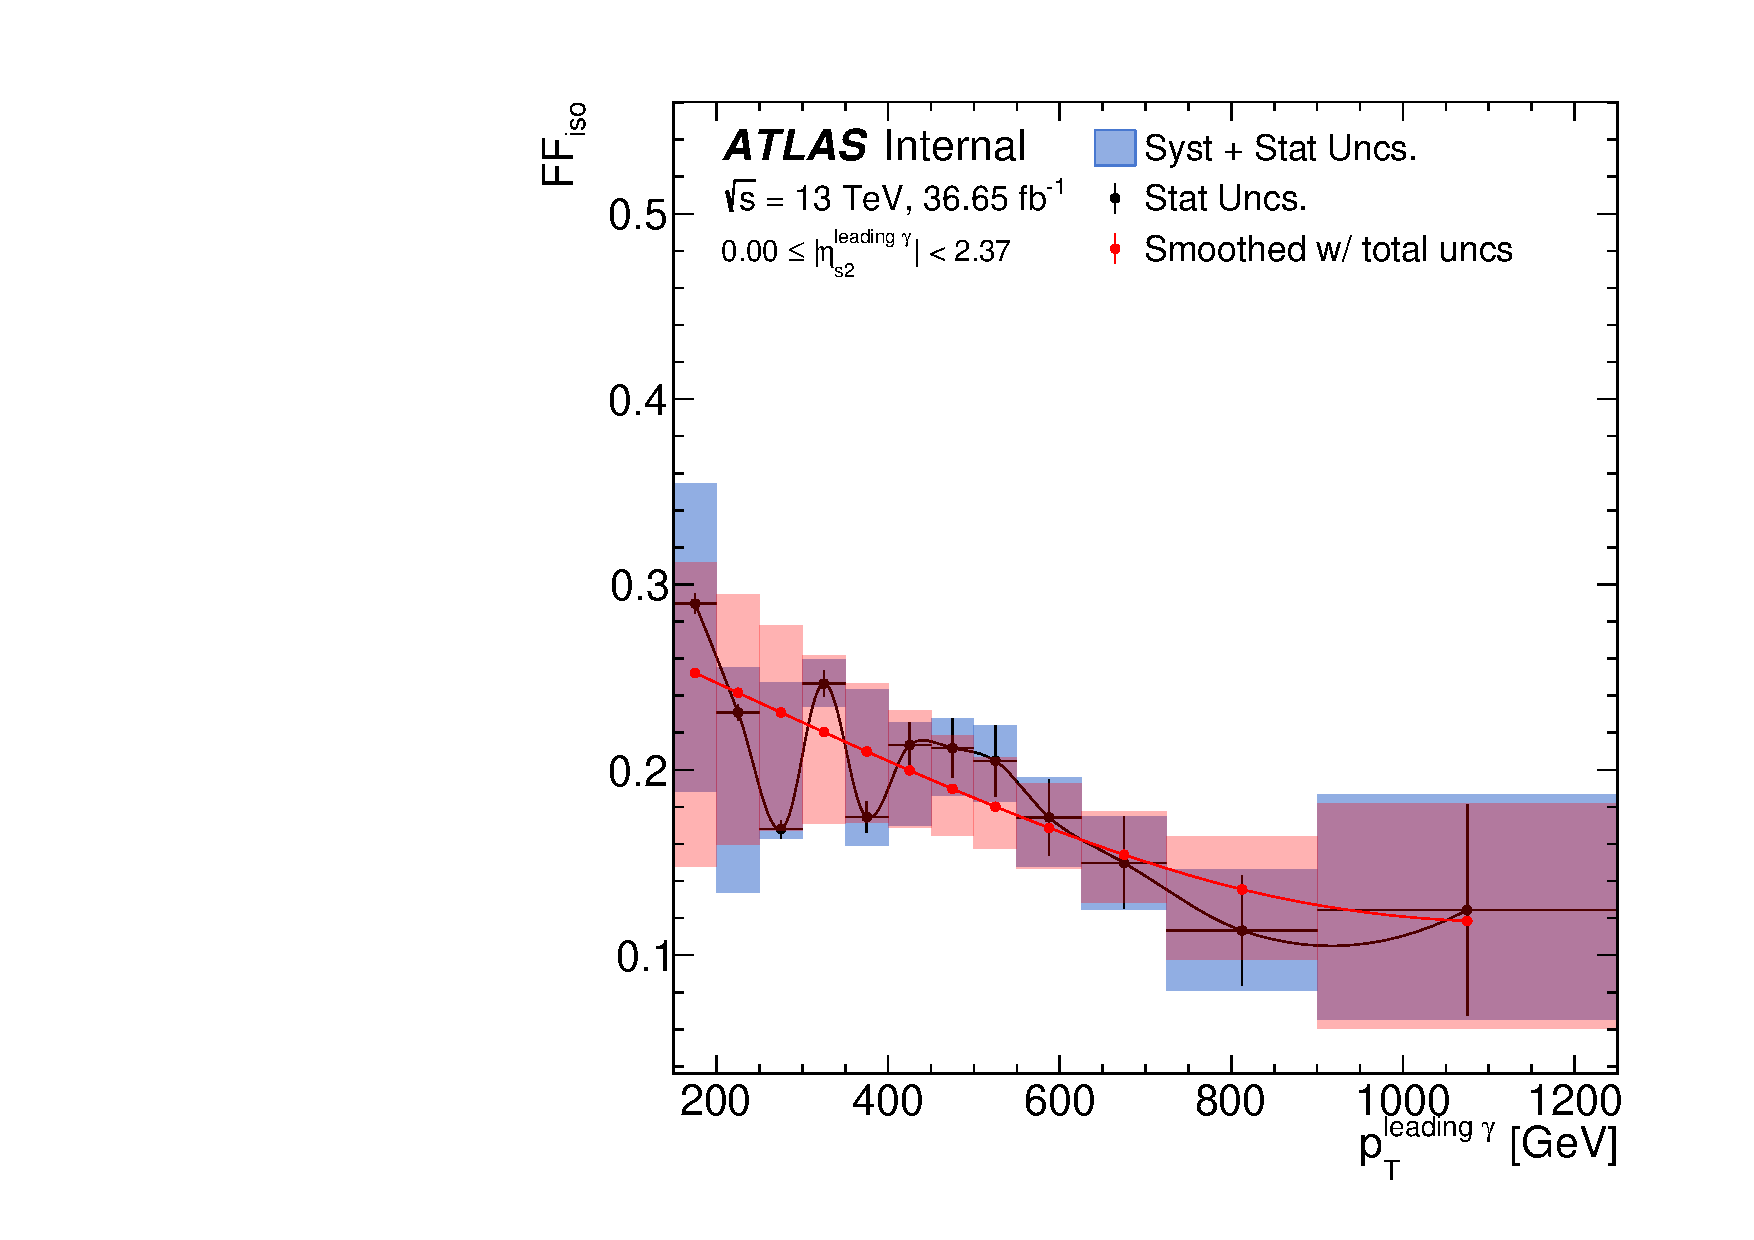
\includegraphics[width=\linewidth]{5_resonances/bkg/estimation/coefficients/can__FF_iso__withsysts__lph_pt0__abslph_etas20_abslph_etas20__0p00__2015_2016}
        \caption{\ffiso.}
        \label{fig:bkg:estimation:results:results:ffiso}
    \end{subfigure}
    \caption{Valores medidos de la pureza de \gammajet \(P_A\) (izquierda) y de los \ffiso (derecha) como función de \ptgam utilizando el método ABCD. Las medidas se muestran con los puntos negros (sólo con incerteza estadística), las áreas sombreadas de azul muestran la incerteza total (estadística y sistemática añadidas en cuadratura) y los puntos rojos con las áreas sombreadas rojas las medidas suavizadas utilizando una interpolación \textit{spline} de tercer orden.}
    \label{fig:bkg:estimation:results:results}
\end{figure}


Los \acp{FaF}, y en particular \ffiso, se aplican a los eventos de datos en una región de control CRJ-X, que sólo difiere de cualquier región de señal \(X\) en el análisis al requerir fotones no aislados. Los valores de \ffiso, por tanto, pueden interpretarse como la probabilidad de que un jet falsee un fotón en la región \(X\) dada la tasa de fotones falsos en CRJ-X. Los resultados se muestran con los puntos negros en la \Fig{\ref{fig:bkg:estimation:results:results:ffiso}} y las incertezas totales con las áreas sombreadas en azul. Como se desprende en estos resultados, se observan valores \ffiso inestables para \(\ptgam<400~\gev\) lo que puede llevar a bumps espurios introducidos por el propio método. Para ello, los valores fueron interpolados utilizando un método de \textit{spline} de tercer orden. Los valores numéricos de los \ffiso se muestran en la \Tab{\ref{tab:bkg:estimation:results:ffiso_purity_values}}.